\chapter{Literaturanalyse} % (fold)
\label{sec:analyse}
In diesem Kapitel werden die in der Einleitung definierten Forschungsfragen untersucht, wofür eine Literaturanalyse erfolgt, die bestehende Studien, Bücher und wissenschaftliche Artikel betrachtet. Ziel ist es, aus der vorhandenen Literatur systematisch Erkenntnisse abzuleiten, die die Performance in verschiedenen Szenarien beleuchten.

\section{Latenzzeit von GraphQL und REST bei unterschiedlichen Anfragenkomplexitäten} % (fold)
\label{sec:ff1}
Um zu untersuchen, wie sich GraphQL und REST in Bezug auf die Latenz bei verschiedenen Anfragekomplexitäten verhalten, ist zunächst darauf einzugehen, welche von den APIs genutzten Faktoren oder Spezifikationen sich auf die Latenz auswirken. Bei der Bereitstellung von Daten setzt REST auf HTTP-Endpunkte, die nativ HTTP-Caching unterstützen, wodurch Ressourcen in einem Cache zwischengespeichert werden können, um unnötige Datenübertragungen sowie Serveranfragen zu vermeiden und somit die Zugriffszeiten zu verringern. Bei GraphQL wird dies nativ nicht unterstützt, wodurch wiederkehrende Anfragen nicht gecacht werden, sondern jeweils vom Server bearbeitet werden müssen, was zu höheren Zugriffszeiten führt.  \citep{graphqlreplacerest}

\noindent
Bei REST wird die Zerlegung von Systemen in eine Menge verknüpfter Ressourcen mit einem bestimmten Granularitätsgrad gefördert, was zu Abwägungen zwischen Wiederverwendbarkeit und Leistung führt, die in der allgemeinen Software-Service-Architektur weitverbreitet sind. Weniger granulare und kohäsivere Services werden bevorzugt, weil sie lose Kopplung und hohe Wiederverwendbarkeit fördern. Dies kann jedoch zu Client-Server-Interaktionen führen, bei denen mehrere aufeinanderfolgende Anfragen notwendig sind, um die benötigten Daten aus dem Ressourcengraphen abzurufen. Dieses Phänomen ist als ‚Underfetching‘ oder ‚n+1-Problem‘ bekannt und tritt bei REST auf der Seite des Clients auf. Dieser muss dementsprechend weitere Anfragen schicken, bis die benötigten Daten vollständig bei ihm verfügbar sind.  \citep{graphqlhealth} \citep{migrategraphql}

\noindent
Bei GraphQL kann es ebenso zu einem n+1-Problem kommen, wobei dieses jedoch nicht auf der Clientseite auftritt, sondern beim Server im Rahmen der Verarbeitung der Anfrage. Der GraphQL-Server muss mehrere Anfragen an die Datenbank schicken, um die benötigten Daten zu erhalten und, an den Client auszuliefern. 
\citep{graphqlsemantics}

\noindent
Hierfür bietet GraphQL einen sogenannten Dataloader, der die zur Bearbeitung eines Requests benötigten Anfragen bündelt und als eine einzelne, optimierte, Datenbankabfrage ausführt. \citep{nordstrom2022graphql}
\newpage
\noindent
Zudem spielt bei der Latenz einer API die Anfragekomplexität eine entscheidende Rolle. In Abbildung 3.1 sind vergleichend die Ausführungszeiten vier unterschiedlicher API-Abfragen dargestellt, die sowohl mit REST als auch mit GraphQL auf den öffentlich zugänglichen GitHub-REST- und GraphQL-APIs durchgeführt wurden. Die Performance wurde hierbei in Millisekunden gemessen und gibt Aufschluss darüber, wie sich beide Technologien je nach Art der Anfrage verhalten.
\begin{figure}[H]
	\centering
	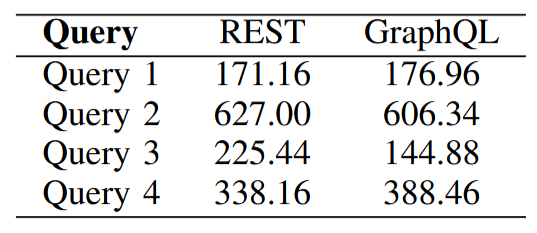
\includegraphics[scale=.5]{Illustrations/cangraphqlreplacerest.png}
\begin{BVerbatim}
Query 1: GET/user
Query 2: POST /repos/:owner/:repo/issues/:issue_number/comments
Query 3: GET/repos/:owner/:repo/issues/:issue_number
Query 4: GET/repos/:owner/:repo/stargazers
\end{BVerbatim}
	\caption{Latenz bei GraphQL vs. REST \citep{graphqlreplacerest}}
\end{figure}
\noindent
Die erste Abfrage (GET/user) zeigt, dass sich die Latenz zwischen REST und GraphQL nicht signifikant unterscheidet: Für diese Anfrage benötigt REST 171,16 Millisekunde, während GraphQL mit 176,96 Millisekunden nur geringfügig langsamer ist. Dies lässt darauf schließen, dass die Ergebnisse bei einfachen Anfragen ohne komplexe Datenstruktur als nahezu identisch bezeichnet werden können. Die zweite Abfrage (POST /repos/:owner/:repo/issues/:issue\_number/comments), eine Schreiboperation, zeigt ein ähnliches Ergebnis, wobei GraphQL mit 606,34 Millisekunden leicht schneller arbeitet als REST mit 627 Millisekunden. Weil der Unterschied gering ist, deutet dies darauf hin, dass Schreiboperationen in beiden Technologien ähnlich effizient verarbeitet werden. 
Eine deutliche Differenz ergibt sich bei der dritten Abfrage (GET/repos/:owner/:repo/issues/:issue\_number), wofür REST 225,44 Millisekunden benötigt, während sich GraphQL mit nur 144,88 Millisekunden als deutlich schneller erweist. Dies demonstriert die Überlegenheit von GraphQL bei komplexeren Datenanforderungen. Weil GraphQL in der Lage ist, mehrere Datenpunkte in einem einzelnen Aufruf zu bündeln, reduziert es die Anzahl der API-Aufrufe und arbeitet so effizienter. Die vierte Abfrage (GET/repos/:owner/:repo/stargazers) zeigt ein gegensätzliches Bild: Hier ist REST mit 338,16 Millisekunden schneller als GraphQL, das 388,46 Millisekunden benötigt. Dies liegt daran, dass die Abfrage keine komplexe Aggregation von Daten erfordert und der Overhead von GraphQL die Performance negativ beeinflusst. Somit kann festgehalten werden, dass REST in einem Szenario positivere Ergebnisse aufwies als GraphQL, in einem Szenario das Gegenteil der Fall war und beide Technologien in zwei Szenarien ähnliche Resultate erzielten. 
\citep{graphqlreplacerest}
\newpage
\noindent
Weitere Studien zeigen, dass GraphQL bei einfachen Abfragen, die nur einen Endpunkt nutzen, etwa 0,02-mal schneller als REST arbeitet.  \citep{migrategraphql}
\newline
Bei komplexeren Anfragen, die vier Endpunkte umfassen und 1000 Ergebnistupel liefern, verarbeitet eine GraphQL-API die Daten bis zu 16-mal schneller als eine REST-API.\citep{analysegraphql}
\newline
Anspruchsvollere Anfragen mit fünf oder mehr Endpunkten werden von GraphQL bis zu 187-mal schneller erfüllt.\citep{analysewebgraphql}
\newline
Bei steigender Komplexität stellt sich jedoch bei einer Menge von 100 000 Ergebnistupeln heraus, dass eine GraphQL-API in diesem Fall 0,36-\citep{analysegraphql} bis 2,5-mal langsamer arbeitet als eine vergleichbare REST-API \citep{restvsgraphql}.
%section ff1 (end)
\section{Latenz von REST- und GraphQL-APIs bei Graph- und relationalen Datenbanken} % (fold)
\label{sec:ff2}
Weil APIs eine Schnittstelle zwischen einer Datenbank und der Anwendung darstellen, die die Daten aus der Datenbank konsumieren soll, ist die Latenz einer API zwingend von der Bearbeitungszeit einer Anfrage innerhalb der Datenbank abhängig. Hierbei nutzen verschiedene Datenbanktypen jeweilige Methoden, um die angefragten Daten aus der Datenbank bereitzustellen. In dieser Arbeit wird durch die Forschungsfrage ein besonderer Schwerpunkt auf die Verarbeitung anhand der relationalen Algebra sowie der Graphentheorie gelegt. Diese Methoden bieten bei der Verwendung in Anwendungsszenarien Vorteile, führen aber zu Nachteilen hinsichtlich der Effizienz und Zeitersparnis bei der Anfragenbearbeitung. Hierbei zeigt sich bei relationalen Datenbanken, dass diese bei steigender Anzahl an gespeicherten Daten zunehmend langsamere Performance bieten. Wie in Abbildung 3.2 jedoch zu sehen ist, stieg die Menge der im Internet verarbeiteten Daten seit 2010 stetig an; die Prognosen bis ins Jahr 2028 deuten auf einen Trend zu erheblich mehr Daten. Graphdatenbanken können mit solch einem Wachstum effektiver umgehen, weil durch die Nutzung Traversal-basierter Anfragen, die für diese Art von Abfragen optimiert sind, die Menge der Daten innerhalb der Datenbank eine untergeordnete Rolle spielt.  \citep{9677042} \citep{performancenosql}
\begin{figure}[H]
	\centering
	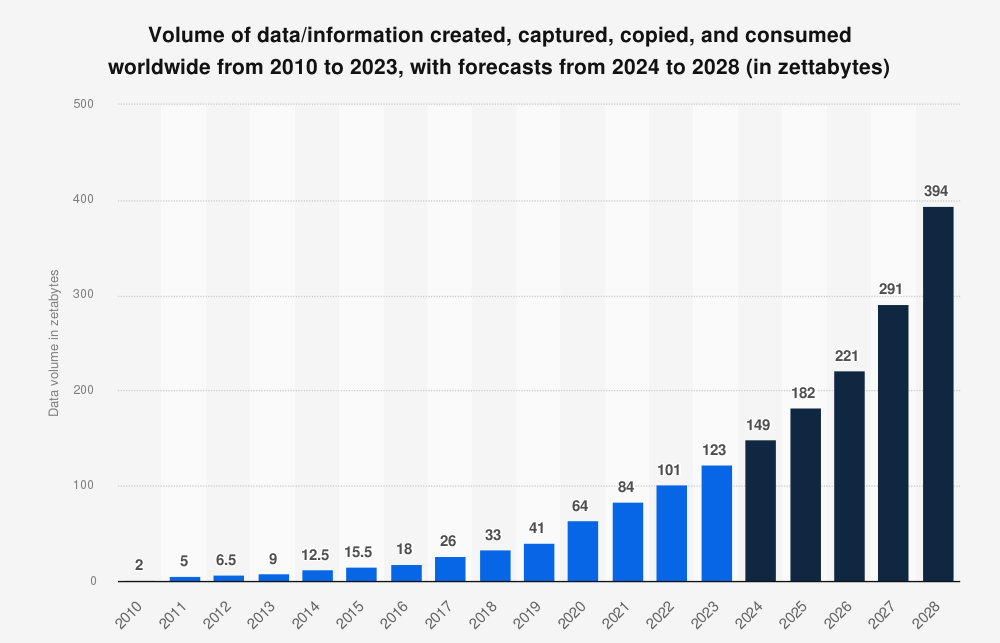
\includegraphics[scale=.4]{Illustrations/growthofdata.png}
	\caption{Datenmenge weltweit \citep{statista}}
\end{figure}
\noindent
Einen weiteren Faktor, der die Performance einer Datenbank beeinflusst, beschreibt die Verbundenheit, also die Relation, der Daten. Abbildung 3.3 zeigt, wie sich diese im Verlauf veränderte. Hierbei ist deutlich zu sehen, dass Daten stetig eine größere Verzweigung zueinander aufweisen.
\begin{figure}[H]
	\centering
	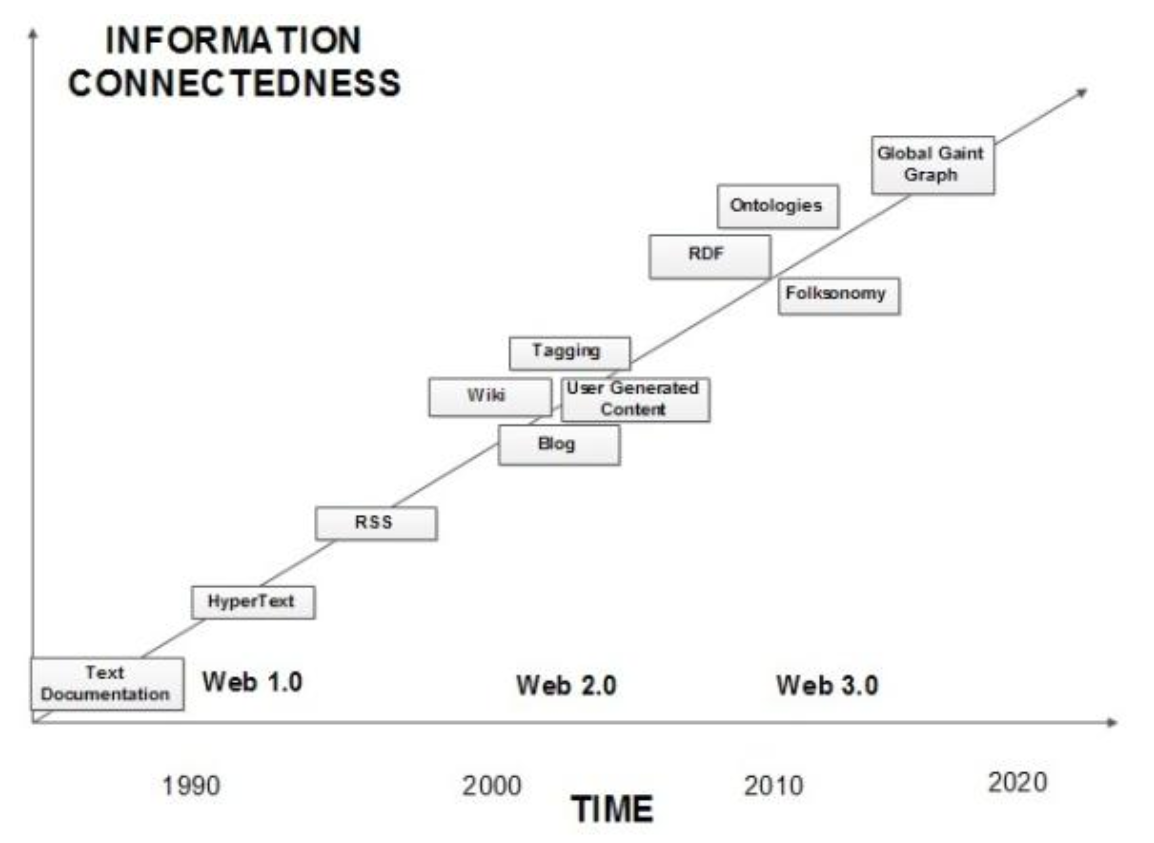
\includegraphics[scale=.45]{Illustrations/informationconnectedness.png}
	\caption{Informationsverbundenheit \citep{performancenosql}}
\end{figure}
\noindent
Eine Graphdatenbank kann mit diesem hohen Grad an Verzweigung durch die Verwendung der Graphentheorie und Traversierung performant umgehen, während bei relationalen Datenbanken dieser hohe Grad der Relationen eine Performanceeinbuße bewirkt. Weil bei der Verbindung der Daten die Relationen zwischen den Tabellen durch Joins realisiert werden und diese komplexer zu berechnen sind, steigt mit zunehmender Anzahl der Relationen die Zeit, welche die Datenbank benötigt, um mithilfe der Schlüssel und mehrerer Tabellen die Beziehung zwischen den Dateneinträgen zu konstruieren.  \citep{9677042} \citep{graphdb}

\noindent
Die Universität von Mississippi führte ein Experiment durch, um die Latenzunterschiede zwischen einer relationalen MySQL- und einer Graphdatenbank (Neo4j) zu untersuchen. Dabei wurden sieben Szenarien simuliert, deren Ergebnisse in den Abbildungen 3.4 und 3.5 dokumentiert sind. In der ersten Spalte der Tabellen wird die Konfiguration der Datenbank dargestellt, wobei die Zahl die Menge der Nodes oder Tupel in der Datenbank angibt, gefolgt von einem Datentyp, der beschreibt, welche Art von Daten bei der Erstellung der Datenbank zufällig verwendet wurde. Die Ergebnisse beider Datenbanken sind in Abbildung 3.4 dargestellt, wobei die Abfragen I1 und I2 unterschiedliche Szenarien repräsentieren: Abfrage I1 selektiert alle Nodes, deren Payload einem bestimmten Wert entspricht, während I2 die Nodes zählt, deren Payload kleiner ist als ein gegebener Wert. Beide Szenarien nutzen den Datentyp Integer, um die Daten anzufordern. Anhand der experimentellen Daten wird deutlich, dass die relationale MySQL-Datenbank im Vergleich zur Graphdatenbank Neo4j in jedem getesteten Fall eine deutlich geringere Latenz aufweist. 
 \citep{graphrelationaldb}
\begin{figure}[H]
	\centering
	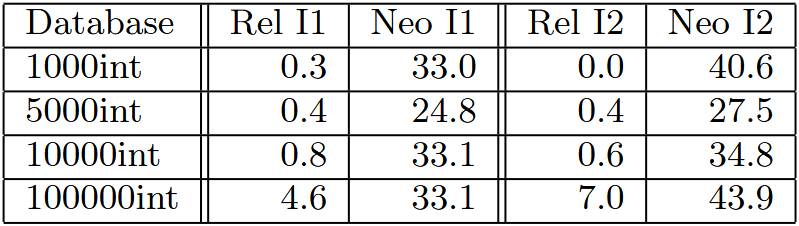
\includegraphics[scale=.5]{Illustrations/dbresultsint.png}
	\caption{Ergebnisse der Abfragen durch Integer in Millisekunden \citep{graphrelationaldb}}
\end{figure}
\noindent
Abbildung 3.5 zeigt Abfragen auf, bei denen anhand eines Strings selektiert wurde, wobei die zweite Zeile angibt, welche Länge der String hatte, auf dessen Basis die Selektion vorgenommen wurde. Hierbei wird die Menge der Nodes gezählt, die den String enthalten. Die Ergebnisse weichen deutlich von den vorherigen Resultaten ab, bei denen mithilfe eines Integer selektiert wurde: Durch die Verwendung eines Strings übertrifft die relationale Datenbank die Graphdatenbank lediglich im ersten Szenario; in den komplexeren Fällen weist die Letztere klare Vorteile auf und ist bei anspruchsvolleren Anfragen in der Spitze um den Faktor 167 schneller. 
 \citep{graphrelationaldb}
\begin{figure}[H]
	\centering
	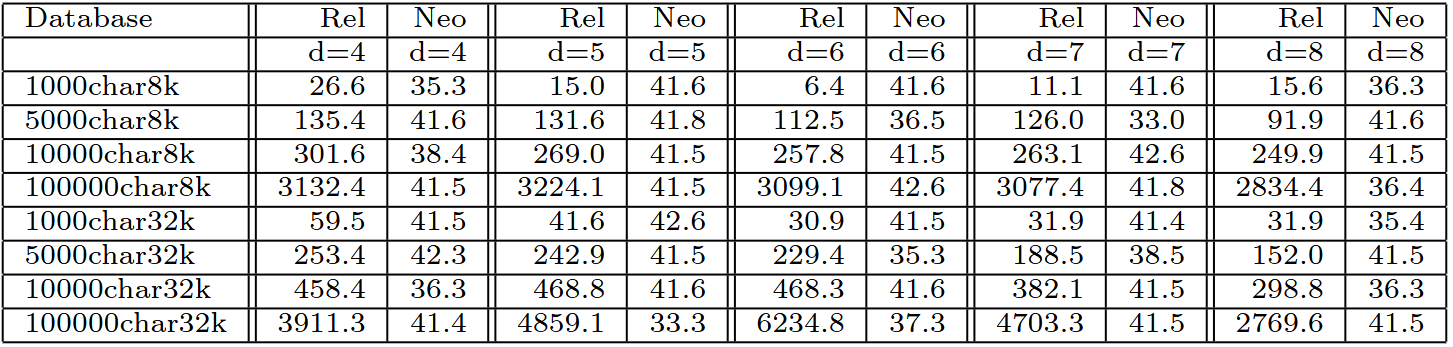
\includegraphics[scale=.425]{Illustrations/dbresultschar.png}
	\caption{Ergebnisse Abfragen durch Character  in Millisekunden \citep{graphrelationaldb}}
\end{figure}
\noindent
Zusammenfassend lässt sich feststellen, dass relationale Datenbanken bei der Selektion von Daten anhand eines Integer deutlich schnellere Ergebnisse liefern. Bei der Abfrage von Daten anhand eines Strings zeigt sich zunächst, dass relationale Datenbanken bei kleinen Daten- mengen effektiver performen, mit zunehmender Datenmenge wird jedoch die Graphdatenbank zunehmend effizienter und übertrifft schließlich die Performance der relationalen Datenbank deutlich.
%section ff2 (end)
% chapter analyse (end)